\documentclass[svgnames,11pt]{beamer}
\input{/home/tof/Documents/Cozy/latex-include/preambule_commun.tex}
\input{/home/tof/Documents/Cozy/latex-include/preambule_beamer.tex}
%\usepackage{pgfpages} \setbeameroption{show notes on second screen=left}
\author[]{Christophe Viroulaud}
\title{Fonction \textbf{\texttt{sorted}}\\Diviser pour régner}
\date{\framebox{\textbf{Algo 01}}}
%\logo{}
\institute{Terminale - NSI}
%DODO trop dur: à retravailler
%DODO prendre algo P49 livre MP2I?
\begin{document}
\begin{frame}
    \titlepage
\end{frame}
\begin{frame}
    \frametitle{}

    En tant que langage de haut niveau, Python offre des méthodes permettant d'effectuer efficacement certaines tâches courantes.\\
    La méthode \textbf{\texttt{sort}} trie en place un tableau.
    \note{tri en place ou nouveau tableau}.
\end{frame}
\begin{frame}
    \frametitle{}

    \begin{framed}
        \centering Quel algorithme de tri est implémenté dans la méthode \textbf{\texttt{sort}}?
    \end{framed}

\end{frame}
\section{Rappel: des algorithmes de tris déjà connus}
\subsection{Tri par sélection}
\begin{frame}[fragile]
    \frametitle{Tri par sélection (en place)}
    \begin{center}
        \begin{lstlisting}[language=Python , basicstyle=\ttfamily\small, xleftmargin=1em, xrightmargin=1em]
Pour chaque élément du tableau
    Trouver le plus petit élément dans la partie non triée.
    Échanger cet élément avec le premier de la partie non triée.
\end{lstlisting}
    \end{center}
    \begin{center}
        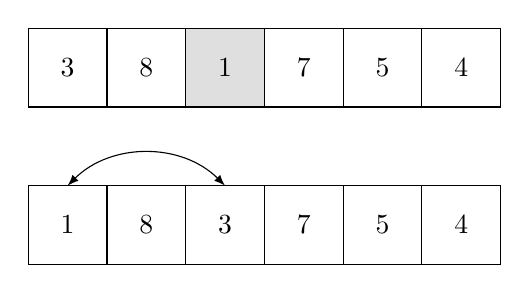
\begin{tikzpicture}

            \node[minimum width=1cm,
                minimum height=1cm,fill=gray!25] at(2.5,2.5) {};
            \draw (0,2) grid (6,3);
            \foreach \k/\i in {3/0,8/1,1/2,7/3,5/4,4/5}
                {\node (\i) at (.5+\i,2.5) {\k};}

            \draw (0,0) grid (6,1);
            \foreach \k/\i in {1/0,8/1,3/2,7/3,5/4,4/5}
                {\node (\i) at (.5+\i,.5) {\k};}
            \draw[<->,>=latex] (0.5,1) to[bend left=45] (2.5,1);
        \end{tikzpicture}
    \end{center}
\end{frame}
\begin{frame}[fragile]
    \frametitle{Tri par sélection (en place)}
    \begin{center}
        \begin{lstlisting}[language=Python , basicstyle=\ttfamily\small, xleftmargin=1em, xrightmargin=1em]
Pour chaque élément du tableau
    Trouver le plus petit élément dans la partie non triée.
    Échanger cet élément avec le premier de la partie non triée.
\end{lstlisting}
    \end{center}
    \begin{activite}
        \begin{enumerate}
            \item Construire par compréhension un tableau de 10 entiers aléatoires compris entre 1 et 100.
            \item Écrire la fonction \textbf{\texttt{tri\_selection(tab: list) $\rightarrow$ None}} qui trie le tableau en place.
        \end{enumerate}
    \end{activite}
\end{frame}
\begin{frame}[fragile]
    \frametitle{Correction}
    \begin{center}
        \begin{lstlisting}[language=Python , basicstyle=\ttfamily\small, xleftmargin=1em, xrightmargin=1em]
tab = [randint(1, 100) for _ in range(10)]
\end{lstlisting}
        \begin{lstlisting}[language=Python , basicstyle=\ttfamily\small, xleftmargin=1em, xrightmargin=1em]
def tri_selection(tab: list) -> None:
    for i in range(len(tab)):
        # trouver le mini
        i_mini = i
        for j in range(i+1, len(tab)):
            if tab[j] < tab[i_mini]:
                i_mini = j
        # échanger
        tab[i], tab[i_mini] = tab[i_mini], tab[i]
\end{lstlisting}
    \end{center}

\end{frame}
\subsection{Tri par insertion}
\begin{frame}[fragile]
    \frametitle{Tri par insertion (en place)}

    \begin{center}
        \begin{lstlisting}[language=bash, basicstyle=\small, xrightmargin=1em]
Pour chaque élément du tableau
    Tant que l'élément précédent est inférieur
            Permuter les deux éléments
\end{lstlisting}
    \end{center}
    \begin{center}
        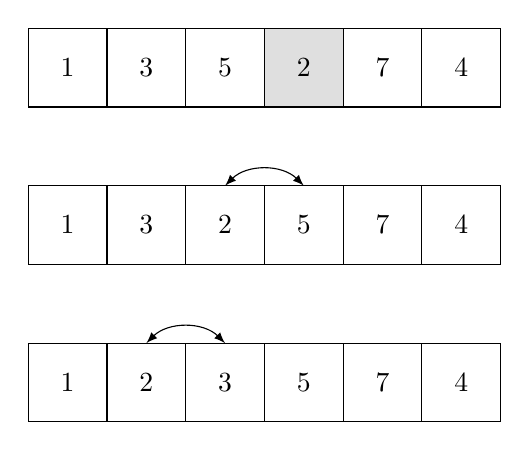
\begin{tikzpicture}
            \node[minimum width=1cm,
                minimum height=1cm,fill=gray!25] at(3.5,2.5) {};
            \draw (0,2) grid (6,3);
            \foreach \k/\i in {1/0,3/1,5/2,2/3,7/4,4/5}
                {\node (\i) at (.5+\i,2.5) {\k};}

            \draw (0,0) grid (6,1);
            \foreach \k/\i in {1/0,3/1,2/2,5/3,7/4,4/5}
                {\node (\i) at (.5+\i,.5) {\k};}
            \draw[<->,>=latex] (2.5,1) to[bend left=45] (3.5,1);
            \draw (0,-2) grid (6,-1);
            \foreach \k/\i in {1/0,2/1,3/2,5/3,7/4,4/5}
                {\node (\i) at (.5+\i,-1.5) {\k};}
            \draw[<->,>=latex] (1.5,-1) to[bend left=45] (2.5,-1);
        \end{tikzpicture}
    \end{center}
\end{frame}
\begin{frame}[fragile]
    \frametitle{Tri par insertion (en place)}

    \begin{center}
        \begin{lstlisting}[language=bash, basicstyle=\small, xrightmargin=1em]
Pour chaque élément du tableau
    Tant que l'élément précédent est inférieur
            Permuter les deux éléments
\end{lstlisting}
    \end{center}
    \begin{activite}
        \begin{enumerate}
            \item Construire par compréhension un tableau de 10 entiers aléatoires compris entre 1 et 100.
            \item Écrire la fonction \textbf{\texttt{tri\_insertion(tab: list) $\rightarrow$ None}} qui trie le tableau en place.
        \end{enumerate}
    \end{activite}
\end{frame}
\begin{frame}[fragile]
    \frametitle{Correction}

    \begin{center}
        \begin{lstlisting}[language=Python , basicstyle=\ttfamily\small, xleftmargin=1em, xrightmargin=1em]
def tri_insertion(tab: list) -> None:
    for i in range(len(tab)-1):
        j = i+1
        # tant que le précédent est inférieur
        while j > 0 and tab[j] < tab[j-1]:
            # permuter
            tab[j], tab[j-1] = tab[j-1], tab[j]
            j -= 1
\end{lstlisting}
    \end{center}
\end{frame}
\subsection{Comparaison des performances}
\begin{frame}
    \frametitle{Comparaison des performances}
    \begin{activite}
        \begin{enumerate}
            \item Construire par compréhension un tableau de 10000 entiers compris entre 1 et 10000.
            \item Mesurer la durée d'exécution de la méthode \textbf{\texttt{sort}} et des deux fonctions précédentes.
        \end{enumerate}
    \end{activite}
    \note{créer un nouveau tableau pour chaque fonction!!}
\end{frame}
\begin{frame}[fragile]
    \frametitle{Correction}

    \begin{center}
        \begin{lstlisting}[language=Python , basicstyle=\ttfamily\small, xleftmargin=2em, xrightmargin=2em]
tab = [randint(1, 10000) for _ in range(10000)]
deb = time()
tri_selection(tab)
fin = time()
print(fin-deb)
\end{lstlisting}
        \captionof{code}{tri par sélection}
        \label{CODE}
    \end{center}
    \begin{center}
        \begin{lstlisting}[language=Python , basicstyle=\ttfamily\small, xleftmargin=2em, xrightmargin=2em]
>>> sélection  4.557838678359985
>>> insertion 3.959839105606079
>>> sort  0.0019469261169433594
\end{lstlisting}
        \captionof{code}{Résultats}
        \label{CODE}
    \end{center}
\end{frame}
\begin{frame}
    \frametitle{Évolution du nombre d'itérations}

    \begin{center}
        \includegraphics[width=9cm]{ressources/complexite-selection.png}
        \captionof{figure}{Tri par sélection: complexité \textbf{quadratique}}
    \end{center}
    \note{15000 éléments $\rightarrow$ 100 millions d'itérations}
\end{frame}
\section{Nouvelle approche}
\subsection{Résoudre de petits problèmes}
\begin{frame}
    \frametitle{Résoudre de petits problèmes}

    \note{La propriété triviale suivante va nous permettre de construire une nouvelle méthode de tri:}
    \begin{aretenir}[Observation]
        Une liste qui contient 0 ou 1 élément est triée.
    \end{aretenir}
    \begin{center}
        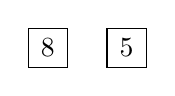
\begin{tikzpicture}[scale=0.5]
            \draw (0,0) -- (1,0) ;
            \draw (1,0) -- (1,1) ;
            \draw (1,1) -- (0,1) ;
            \draw (0,1) -- (0,0) ;

            \draw (2,0) -- (3,0) ;
            \draw (3,0) -- (3,1) ;
            \draw (3,1) -- (2,1) ;
            \draw (2,1) -- (2,0) ;

            \draw (0.5,0.5) node{8};
            \draw (2.5,0.5) node{5};
        \end{tikzpicture}
        \captionof{figure}{Deux listes triées}
    \end{center}

\end{frame}
\begin{frame}
    \frametitle{}

    Deux listes d'un élément chacune peuvent être fusionnées en une liste triée de deux éléments.
    \begin{center}
        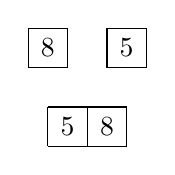
\begin{tikzpicture}[scale=0.5]
            \draw (0.5,-1) -- (2.5,-1) ;
            \draw (2.5,-1) -- (2.5,-2) ;
            \draw (2.5,-2) -- (0.5,-2) ;
            \draw (0.5,-2) -- (0.5,-1) ;
            \draw (1.5,-1) -- (1.5,-2) ;

            \draw (1,-1.5) node{5};
            \draw (2,-1.5) node{8};

            \draw (0,0) -- (1,0) ;
            \draw (1,0) -- (1,1) ;
            \draw (1,1) -- (0,1) ;
            \draw (0,1) -- (0,0) ;

            \draw (2,0) -- (3,0) ;
            \draw (3,0) -- (3,1) ;
            \draw (3,1) -- (2,1) ;
            \draw (2,1) -- (2,0) ;

            \draw (0.5,0.5) node{8};
            \draw (2.5,0.5) node{5};
        \end{tikzpicture}
        \captionof{figure}{Fusionner 2 listes de 1 élément}

    \end{center}

\end{frame}
\begin{frame}
    \frametitle{}

    \begin{aretenir}[Principe]
        En résolvant des petits problèmes, nous pouvons remonter à des problèmes plus importants en appliquant le même principe.
    \end{aretenir}

\end{frame}
\subsection{...pour solutionner un gros problème}
\begin{frame}
    \frametitle{...pour solutionner un gros problème}

    \begin{center}
        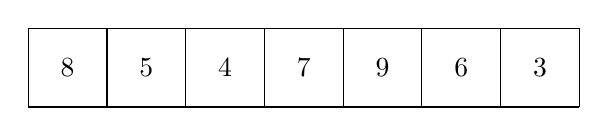
\begin{tikzpicture}
            \draw (0,0) grid (7,1);
            \foreach \k/\i in {8/0,5/1,4/2,7/3,9/4,6/5,3/6}
                {\node (\i) at (.5+\i,.5) {\k};}
        \end{tikzpicture}
        \captionof{figure}{Un gros problème: trier une liste}
    \end{center}
    \note{essayons de nous ramener à de petits problèmes}
\end{frame}
\begin{frame}
    \frametitle{}
    \note{Pour se ramener à un problème plus petit, séparons la liste en deux listes}
    \begin{center}
        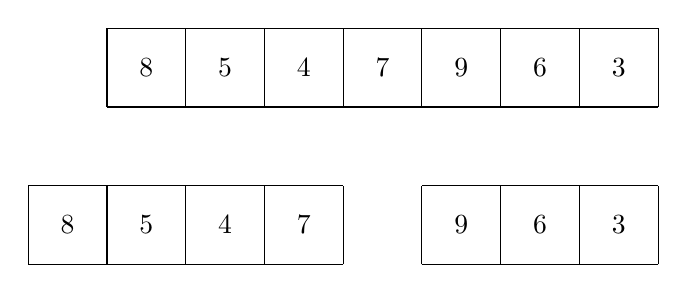
\begin{tikzpicture}
            \draw (0,0) grid (7,1);
            \foreach \k/\i in {8/0,5/1,4/2,7/3,9/4,6/5,3/6}
                {\node (\i) at (.5+\i,.5) {\k};}
            \draw (-1,-2) grid (3,-1);
            \foreach \k/\i in {8/0,5/1,4/2,7/3}
                {\node (\i) at (-.5+\i,-1.5) {\k};}
            \draw (4,-2) grid (7,-1);
            \foreach \k/\i in {9/0,6/1,3/2}
                {\node (\i) at (4.5+\i,-1.5) {\k};}
        \end{tikzpicture}
        \captionof{figure}{Séparer la liste en deux listes plus petites}
    \end{center}

\end{frame}
\begin{frame}
    \frametitle{}
    \begin{center}
        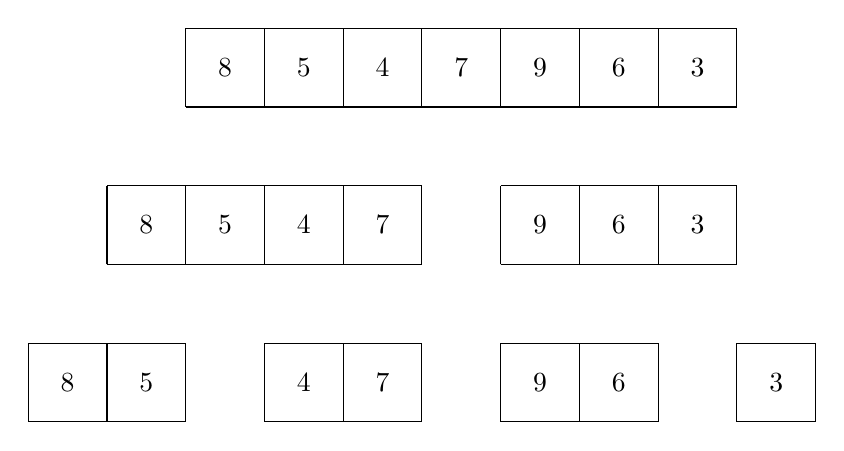
\begin{tikzpicture}
            \draw (0,0) grid (7,1);
            \foreach \k/\i in {8/0,5/1,4/2,7/3,9/4,6/5,3/6}
                {\node (\i) at (.5+\i,.5) {\k};}

            \draw (-1,-2) grid (3,-1);
            \foreach \k/\i in {8/0,5/1,4/2,7/3}
                {\node (\i) at (-.5+\i,-1.5) {\k};}
            \draw (4,-2) grid (7,-1);
            \foreach \k/\i in {9/0,6/1,3/2}
                {\node (\i) at (4.5+\i,-1.5) {\k};}

            \draw (-2,-4) grid (0,-3);
            \foreach \k/\i in {8/0,5/1}
                {\node (\i) at (-1.5+\i,-3.5) {\k};}
            \draw (1,-4) grid (3,-3);
            \foreach \k/\i in {4/0,7/1}
                {\node (\i) at (1.5+\i,-3.5) {\k};}
            \draw (4,-4) grid (6,-3);
            \foreach \k/\i in {9/0,6/1}
                {\node (\i) at (4.5+\i,-3.5) {\k};}
            \draw (7,-4) grid (8,-3);
            \foreach \k/\i in {3/0}
                {\node (\i) at (7.5+\i,-3.5) {\k};}

        \end{tikzpicture}
    \end{center}

\end{frame}
\begin{frame}
    \frametitle{}
    \begin{center}
        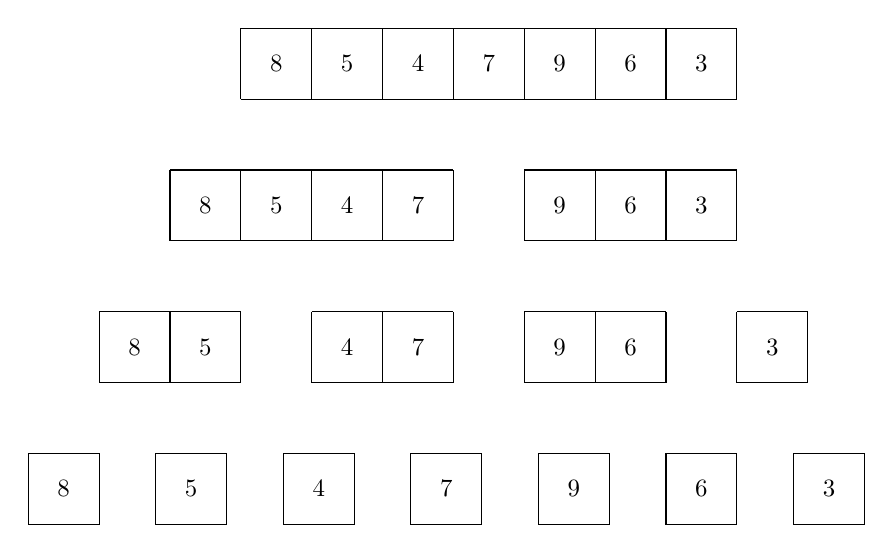
\begin{tikzpicture}[scale=0.9, transform shape]
            \draw (0,0) grid (7,1);
            \foreach \k/\i in {8/0,5/1,4/2,7/3,9/4,6/5,3/6}
                {\node (\i) at (.5+\i,.5) {\k};}

            \draw (-1,-2) grid (3,-1);
            \foreach \k/\i in {8/0,5/1,4/2,7/3}
                {\node (\i) at (-.5+\i,-1.5) {\k};}
            \draw (4,-2) grid (7,-1);
            \foreach \k/\i in {9/0,6/1,3/2}
                {\node (\i) at (4.5+\i,-1.5) {\k};}

            \draw (-2,-4) grid (0,-3);
            \foreach \k/\i in {8/0,5/1}
                {\node (\i) at (-1.5+\i,-3.5) {\k};}
            \draw (1,-4) grid (3,-3);
            \foreach \k/\i in {4/0,7/1}
                {\node (\i) at (1.5+\i,-3.5) {\k};}
            \draw (4,-4) grid (6,-3);
            \foreach \k/\i in {9/0,6/1}
                {\node (\i) at (4.5+\i,-3.5) {\k};}
            \draw (7,-4) grid (8,-3);
            \foreach \k/\i in {3/0}
                {\node (\i) at (7.5+\i,-3.5) {\k};}


            \foreach \k/\i in {8/0,5/1,4/2,7/3,9/4,6/5,3/6}
                {\node[minimum width=1cm,
                        minimum height=1cm,draw] (\i) at (-2.5+1.8*\i,-5.5) {\k};}
        \end{tikzpicture}
        \captionof{figure}{Obtenir de petits problèmes}
    \end{center}

\end{frame}
\begin{frame}
    \frametitle{}
    \begin{center}
        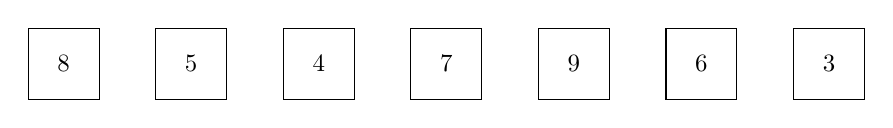
\begin{tikzpicture} [scale=0.9, transform shape]
            \foreach \k/\i in {8/0,5/1,4/2,7/3,9/4,6/5,3/6}
                {\node[minimum width=1cm,
                        minimum height=1cm,draw] (\i) at (-2.5+1.8*\i,-5.5) {\k};}
        \end{tikzpicture}
        \captionof{figure}{Résoudre les petits problèmes}
    \end{center}

\end{frame}
\begin{frame}
    \frametitle{}
    \begin{center}
        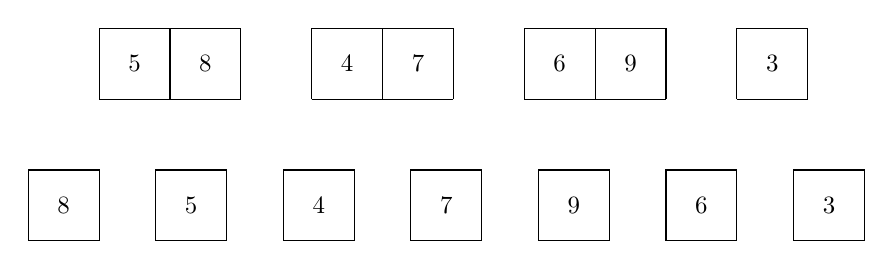
\begin{tikzpicture}[scale=0.9, transform shape]

            \draw (-2,-4) grid (0,-3);
            \foreach \k/\i in {5/0,8/1}
                {\node (\i) at (-1.5+\i,-3.5) {\k};}
            \draw (1,-4) grid (3,-3);
            \foreach \k/\i in {4/0,7/1}
                {\node (\i) at (1.5+\i,-3.5) {\k};}
            \draw (4,-4) grid (6,-3);
            \foreach \k/\i in {6/0,9/1}
                {\node (\i) at (4.5+\i,-3.5) {\k};}
            \draw (7,-4) grid (8,-3);
            \foreach \k/\i in {3/0}
                {\node (\i) at (7.5+\i,-3.5) {\k};}


            \foreach \k/\i in {8/0,5/1,4/2,7/3,9/4,6/5,3/6}
                {\node[minimum width=1cm,
                        minimum height=1cm,draw] (\i) at (-2.5+1.8*\i,-5.5) {\k};}
        \end{tikzpicture}
        \captionof{figure}{Trier...}
    \end{center}

\end{frame}

\begin{frame}
    \frametitle{}
    \begin{center}
        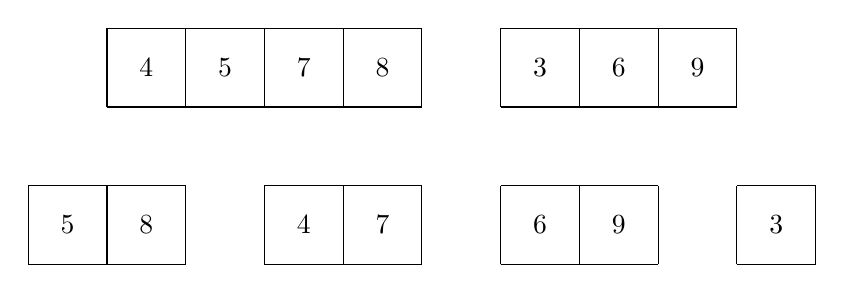
\begin{tikzpicture}
            \draw (-1,-2) grid (3,-1);
            \foreach \k/\i in {4/0,5/1,7/2,8/3}
                {\node (\i) at (-.5+\i,-1.5) {\k};}
            \draw (4,-2) grid (7,-1);
            \foreach \k/\i in {3/0,6/1,9/2}
                {\node (\i) at (4.5+\i,-1.5) {\k};}

            \draw (-2,-4) grid (0,-3);
            \foreach \k/\i in {5/0,8/1}
                {\node (\i) at (-1.5+\i,-3.5) {\k};}
            \draw (1,-4) grid (3,-3);
            \foreach \k/\i in {4/0,7/1}
                {\node (\i) at (1.5+\i,-3.5) {\k};}
            \draw (4,-4) grid (6,-3);
            \foreach \k/\i in {6/0,9/1}
                {\node (\i) at (4.5+\i,-3.5) {\k};}
            \draw (7,-4) grid (8,-3);
            \foreach \k/\i in {3/0}
                {\node (\i) at (7.5+\i,-3.5) {\k};}

        \end{tikzpicture}
        \captionof{figure}{\dots et remonter}
    \end{center}

\end{frame}
\begin{frame}
    \frametitle{}
    \begin{center}
        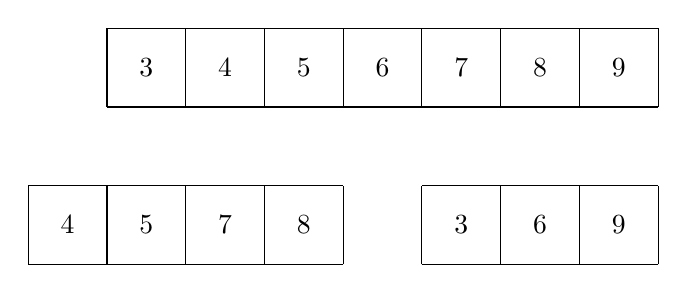
\begin{tikzpicture}
            \draw (0,0) grid (7,1);
            \foreach \k/\i in {3/0,4/1,5/2,6/3,7/4,8/5,9/6}
                {\node (\i) at (.5+\i,.5) {\k};}

            \draw (-1,-2) grid (3,-1);
            \foreach \k/\i in {4/0,5/1,7/2,8/3}
                {\node (\i) at (-.5+\i,-1.5) {\k};}
            \draw (4,-2) grid (7,-1);
            \foreach \k/\i in {3/0,6/1,9/2}
                {\node (\i) at (4.5+\i,-1.5) {\k};}
        \end{tikzpicture}
        \captionof{figure}{Le tri se termine}
    \end{center}

\end{frame}
\subsection{Diviser pour régner: un algorithme récursif}
\begin{frame}
    \frametitle{Diviser pour régner: un algorithme récursif}
    \begin{center}
        \begin{itemize}
            \item \textbf{cas limite:} la liste est de taille minimale
            \item sinon
                  \begin{itemize}
                      \item on coupe la liste en 2,
                      \item \textbf{appel récursif} sur chaque liste
                      \item \textbf{fusionner} les listes lors de la remontée d'appel
                  \end{itemize}
        \end{itemize}
        \captionof{code}{Tri fusion}
    \end{center}
\end{frame}
\begin{frame}
    \begin{center}
        \begin{itemize}
            \item \textbf{cas limite:} la liste est de taille minimale
            \item sinon
                  \begin{itemize}
                      \item on coupe la liste en 2,
                      \item \textbf{appel récursif} sur chaque liste
                      \item \textbf{fusionner} les listes lors de la remontée d'appel
                  \end{itemize}
        \end{itemize}
        \captionof{code}{Tri fusion}
    \end{center}
    \begin{activite}
        Soit la fonction \textbf{\texttt{fusionner(tab: list, deb: int, fin: int) $\rightarrow$ None}} qui trie les éléments de \textbf{\texttt{tab}} entre les indices \textbf{\texttt{deb}} et \textbf{\texttt{fin}}.\\ Écrire la fonction \textbf{\texttt{tri\_fusion(tab: list, deb: int, fin: int) $\rightarrow$ None}} qui trie le tableau \emph{en place}.
    \end{activite}

\end{frame}
\begin{frame}[fragile]
    \frametitle{Correction}

    \begin{center}
        \begin{lstlisting}[language=Python , basicstyle=\ttfamily\small, xleftmargin=1em, xrightmargin=1em]
def tri_fusion(tab: list, deb: int, fin: int) -> None:
if deb < fin:
    milieu = (deb+fin)//2
    tri_fusion(tab, deb, milieu)
    tri_fusion(tab, milieu+1, fin)
    fusionner(tab, deb, fin)
\end{lstlisting}
        \captionof{code}{Tri fusion}
        \label{CODE}
    \end{center}

\end{frame}
\subsection{Étape de la fusion}
\begin{frame}
    \frametitle{Étape de la fusion}

    Lors de la remontée d'appel, la \emph{fusion} assemble deux tableaux triés en un seul.
    \begin{center}
        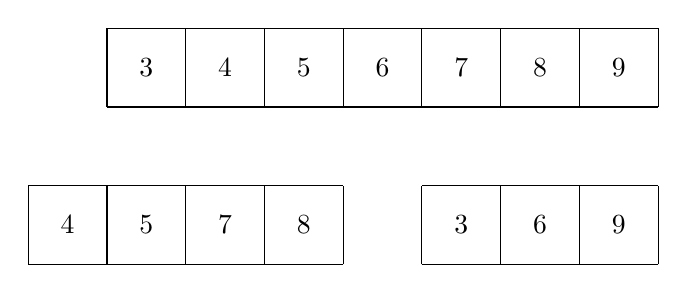
\begin{tikzpicture}
            \draw (0,0) grid (7,1);
            \foreach \k/\i in {3/0,4/1,5/2,6/3,7/4,8/5,9/6}
                {\node (\i) at (.5+\i,.5) {\k};}

            \draw (-1,-2) grid (3,-1);
            \foreach \k/\i in {4/0,5/1,7/2,8/3}
                {\node (\i) at (-.5+\i,-1.5) {\k};}
            \draw (4,-2) grid (7,-1);
            \foreach \k/\i in {3/0,6/1,9/2}
                {\node (\i) at (4.5+\i,-1.5) {\k};}
        \end{tikzpicture}
        \captionof{figure}{Fusionner}
    \end{center}

\end{frame}
\begin{frame}
    \frametitle{}

    En pratique, nous effectuons un tri \emph{place}.
    \begin{center}
        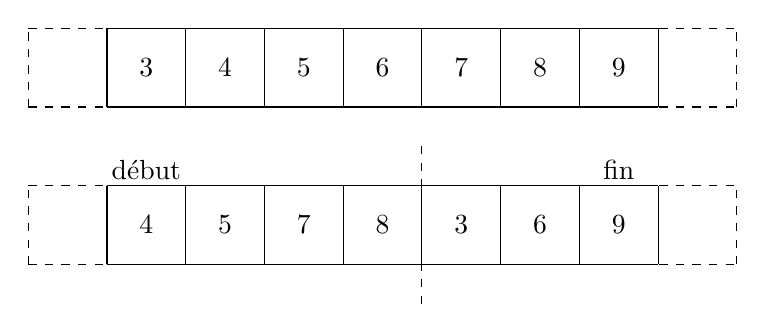
\begin{tikzpicture}
            \node at(.5,-.8) {début};
            \node at(6.5,-.8) {fin};
            \draw[dashed] (4,-2.5) -- (4,-.5);
            \draw[dashed] (-1,0) grid (8,1);
            \draw (0,0) grid (7,1);
            \foreach \k/\i in {3/0,4/1,5/2,6/3,7/4,8/5,9/6}
                {\node (\i) at (.5+\i,.5) {\k};}

            \draw[dashed] (-1,-2) grid (8,-1);
            \draw (0,-2) grid (7,-1);
            \foreach \k/\i in {4/0,5/1,7/2,8/3,3/4,6/5,9/6}
                {\node (\i) at (.5+\i,-1.5) {\k};}
        \end{tikzpicture}
        \captionof{figure}{Fusionner}
    \end{center}
\end{frame}

\begin{frame}
    \frametitle{}

    Pour assembler les deux parties du tableau, il faut prendre le plus petit élément, jusqu'à vider un des deux blocs. Puis on complète avec les éléments restants.

    \begin{center}
        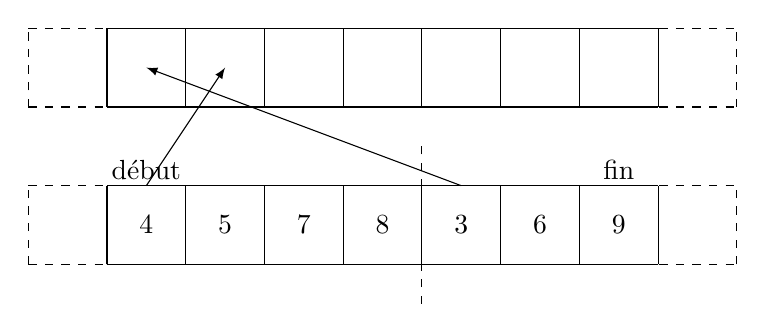
\begin{tikzpicture}
            \node at(.5,-.8) {début};
            \node at(6.5,-.8) {fin};
            \draw[dashed] (4,-2.5) -- (4,-.5);
            \draw[dashed] (-1,0) grid (8,1);
            \draw (0,0) grid (7,1);

            \draw[dashed] (-1,-2) grid (8,-1);
            \draw (0,-2) grid (7,-1);
            \foreach \k/\i in {4/0,5/1,7/2,8/3,3/4,6/5,9/6}
                {\node (\i) at (.5+\i,-1.5) {\k};}

            \draw[->,>=latex] (4.5,-1) to (.5,.5);
            \draw[->,>=latex] (.5,-1) to (1.5,.5);
        \end{tikzpicture}
        \captionof{figure}{Fusionner}
    \end{center}
\end{frame}
\begin{frame}
    \frametitle{}

    Puis on complète avec les éléments restants.

    \begin{center}
        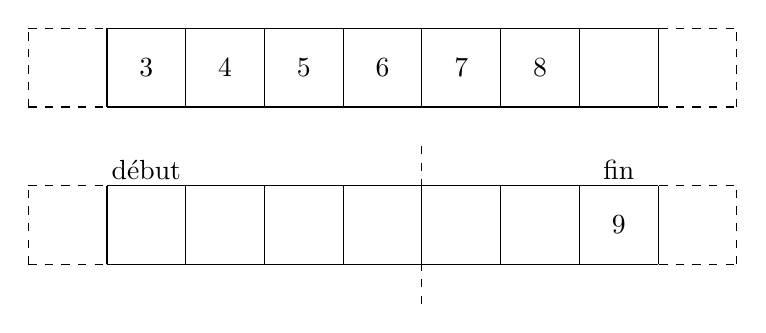
\begin{tikzpicture}
            \node at(.5,-.8) {début};
            \node at(6.5,-.8) {fin};
            \draw[dashed] (4,-2.5) -- (4,-.5);
            \draw[dashed] (-1,0) grid (8,1);
            \draw (0,0) grid (7,1);
            \foreach \k/\i in {3/0,4/1,5/2,6/3,7/4,8/5}
                {\node (\i) at (.5+\i,.5) {\k};}
            \draw[dashed] (-1,-2) grid (8,-1);
            \draw (0,-2) grid (7,-1);
            \foreach \k/\i in {9/6}
                {\node (\i) at (.5+\i,-1.5) {\k};}
        \end{tikzpicture}
        \captionof{figure}{Compléter}
    \end{center}
    \begin{aretenir}[Remarque]
        En pratique nous utiliserons un tableau temporaire pour fusionner.
    \end{aretenir}
\end{frame}
\begin{frame}
    \frametitle{}

    \begin{activite}
        Écrire la fonction \textbf{\texttt{fusionner(tab: list, deb: int, fin: int) $\rightarrow$ None}} qui assemble les éléments de \textbf{\texttt{tab}} entre les indices \textbf{\texttt{deb}} et \textbf{\texttt{fin}}. Les éléments seront d'abord stockés dans un tableau temporaire qui viendra ensuite écraser la partie de \textbf{\texttt{tab}}.
    \end{activite}

\end{frame}
\begin{frame}[fragile]
    \frametitle{Correction}

    \begin{center}
        \begin{lstlisting}[language=Python , basicstyle=\ttfamily\small, xleftmargin=1em, xrightmargin=1em]
def fusionner(tab: list, deb: int, fin: int) -> None:
    res = [0 for _ in range(fin-deb+1)]
    milieu = (deb+fin)//2
    i = deb
    j = milieu+1
    k = 0
\end{lstlisting}
        \captionof{code}{initialiser}
        \label{CODE}
    \end{center}

\end{frame}
\begin{frame}[fragile]
    \frametitle{Correction}

    \begin{center}
        \begin{lstlisting}[language=Python , basicstyle=\ttfamily\small, xleftmargin=1em, xrightmargin=1em]
while i <= milieu and j <= fin:
    if tab[i] < tab[j]:
        res[k] = tab[i]
        i += 1
    else:
        res[k] = tab[j]
        j += 1
    k += 1
\end{lstlisting}
        \captionof{code}{assembler}
        \label{CODE}
    \end{center}

\end{frame}
\begin{frame}[fragile]
    \frametitle{Correction}

    \begin{center}
        \begin{lstlisting}[language=Python , basicstyle=\ttfamily\small, xleftmargin=1em, xrightmargin=1em]
for i1 in range(i, milieu+1):
    res[k] = tab[i1]
    k += 1
for j1 in range(j, fin+1):
    res[k] = tab[j1]
    k += 1
\end{lstlisting}
        \captionof{code}{compléter}
        \label{CODE}
    \end{center}

\end{frame}
\begin{frame}[fragile]
    \frametitle{Correction}

    \begin{center}
        \begin{lstlisting}[language=Python , basicstyle=\ttfamily\small, xleftmargin=1em, xrightmargin=1em]
# remplacement tab par res
for k in range(fin-deb+1):
    tab[deb+k] = res[k]
\end{lstlisting}
        \captionof{code}{remplacer}
        \label{CODE}
    \end{center}

\end{frame}
\section{Performances du tri fusion}
\subsection{Mesure de la durée d'exécution}
\begin{frame}
    \frametitle{Mesure de la durée d'exécution}

    \begin{activite}
        \begin{enumerate}
            \item Construire par compréhension un tableau de 10000 entiers compris entre 1 et 10000.
            \item Mesurer la durée d'exécution de la fonction \textbf{\texttt{tri\_fusion}} et des deux fonctions précédentes.
        \end{enumerate}
    \end{activite}

\end{frame}
\begin{frame}[fragile]
    \frametitle{Correction}

    \begin{center}
        \begin{lstlisting}[language=Python , basicstyle=\ttfamily\small, xleftmargin=2em, xrightmargin=2em]
tab = [randint(1, 10000) for _ in range(10000)]
deb = time()
tri_fusion(tab2, 0, len(tab)-1)
fin = time()
print("fusion ", fin-deb)
\end{lstlisting}
        \begin{lstlisting}[language=Python , basicstyle=\ttfamily\small, xleftmargin=2em, xrightmargin=2em]
>>> sélection  4.557838678359985
>>> insertion 3.959839105606079
>>> sort  0.0019469261169433594
>>> fusion  0.1485743522644043
\end{lstlisting}
    \end{center}

\end{frame}
\subsection{Complexité}
\begin{frame}
    \frametitle{Complexité du découpage}


    \begin{itemize}
        \item<1-> À chaque appel de la fonction \texttt{\textbf{tri\_fusion}} nous divisons la liste en deux.
        \item<2-> Combien de fois faut-il couper la liste en deux pour obtenir des listes d'un élément?
    \end{itemize}

\end{frame}
\begin{frame}
    \frametitle{}

    \begin{center}
        Mathématiquement nous cherchons \emph{a} tel que: {\Large $$\dfrac{n}{2^a}=1$$}
    \end{center}



\end{frame}
\begin{frame}
    \frametitle{}
    Le logarithme base 2 noté $log_2$ se définit: $log_2(2^x)=x$.
    $$\dfrac{n}{2^a}=1$$
    $$\Longleftrightarrow n=2^a$$
    $$\Longleftrightarrow \log_2 n = \log_2 (2^a)$$
    $$\Longleftrightarrow \log_2 n = a$$

    \begin{aretenir}[]
        La complexité du découpage en sous-listes est \textbf{logarithmique}.
    \end{aretenir}
\end{frame}
\begin{frame}
    \frametitle{Complexité de la fusion}

    La fonction \textbf{\texttt{fusionner}} réalise \emph{n} comparaisons pour assembler deux listes de taille $\dfrac{n}{2}$.
\note{qq soit le niveau, pour fusionner on se contente de parcourir une fois un tableau}

\end{frame}
\begin{frame}
    \frametitle{}
    \begin{center}
        \begin{tikzpicture}
            \node[draw, minimum height=.7cm,minimum width = .7cm] (50) at (2.45,8) {n};
            \foreach \i in {0,1}
                {\node[draw, minimum height=.7cm,minimum width = .7cm] (4\i) at (1.05+2.8*\i,6) {$\frac{n}{2}$};}
            \foreach \i/\j in {00/0,01/1,10/2,11/3}
                {\node[draw, minimum height=.7cm,minimum width = .7cm] (3\i) at (.35+1.4*\j,4) {$\frac{n}{4}$};}
            \foreach \i/\j in {000/0,001/1,010/2,011/3,100/4,101/5,110/6,111/7}
                {\node[draw, minimum height=.7cm,minimum width = .7cm] (2\i) at (.7*\j,2) {$\frac{n}{8}$};}
            \draw (2,1) node{.........};
            \foreach \i in {0,1,...,9}
                {\node[draw, minimum height=.7cm,minimum width = .7cm] (\i) at (-.7+.7*\i,0) {1};}

            \foreach \i in {0,1}
                {\draw (50.south) -- (4\i.north);}
            \foreach \i in {0,1}{
                \foreach \j in {0,1}
                {\draw (4\i.south) -- (3\i\j.north);}
                }
            \foreach \i in {00,01,10,11}{
                \foreach \j in {0,1}
                {\draw (3\i.south) -- (2\i\j.north);}
                }
            
                \draw (8,8) node{$n$};
                \draw (8,6) node{$2×(\dfrac{n}{2})=n$};
                \draw (8,4) node{$2^2×(\dfrac{n}{2^2})=n$};
                \draw (8,2) node{$2^3×(\dfrac{n}{2^3})=n$};
                \draw (8,0) node{$2^{log_2(n)}×(\dfrac{n}{2^{log_2(n)}})=n$};
    
        \end{tikzpicture}
    \end{center}


\end{frame}
\begin{frame}
    \frametitle{Complexité du tri fusion}

    \begin{aretenir}[]
        Chaque niveau de fusion a un coup de \emph{n} et il y a $\log_2(n)$ niveaux.
        {\Large $$O(n×log_2(n))$$}
    \end{aretenir}

\end{frame}
\begin{frame}
    \frametitle{}

    \begin{activite}
    Sachant que la complexité du tri par sélection est quadratique, la comparer au tri fusion pour un tableau de 100, 1000, 10000, 100000 éléments.
    \end{activite}
$$\log_2(n)=\frac{\ln n}{\ln 2}$$
\end{frame}
\begin{frame}
    \frametitle{Correction}

    \begin{center}
        \begin{tabular}{|*{3}{c|}}
            \hline
            éléments & tri par sélection & tri fusion\\
            \hline
            100&$10^4$&664\\
            \hline
            1000&$10^6$&9966\\
            \hline
            10000&$10^8$&132877\\
            \hline
            100000&$10^{10}$&1660964\\
            \hline
        \end{tabular}
    \end{center}

\end{frame}
\section{Timsort}
\begin{frame}
    \frametitle{Timsort}

La méthode native \textbf{\texttt{sort}} implémente l’algorithme \textbf{Timsort} mis au point par Tim Peters en 2002. C’est un algorithme hybride de plusieurs tris.

\begin{activite}
\textbf{Recherche:}
\begin{itemize}
    \item Donner les algorithmes de tris utilisés dans Timsort.
    \item Détailler dans quel cas est utilisé chacun des tris.
    \item En discutant de la complexité, expliquer pour quelle raison le tri par insertion est plus intéressant que le tri par sélection.
\end{itemize}
\end{activite}
\end{frame}
\end{document}
